\documentclass[a4paper,10pt,twoside]{report}
\usepackage{geometry}\geometry{a4paper,top=3.5cm,bottom=3.5cm,%
left=2.5cm,right=2.5cm,heightrounded,bindingoffset=0mm}
\usepackage[T1]{fontenc}
\usepackage[utf8]{inputenc}
\usepackage[italian]{babel}
\usepackage{graphicx}
\usepackage[export]{adjustbox}%Per il Frame attrono le immagini e il valign
\usepackage{subfig}
\usepackage{amsmath,amsfonts,amssymb,braket,mathrsfs}
\usepackage{float}
\usepackage{tabularx,booktabs}
\usepackage{hyperref}
\usepackage{epsfig}
\usepackage{pdfpages} %Per gli allegati
%\usepackage{minipage}
\usepackage[output-decimal-marker={,}]{siunitx}
\DeclareSIUnit \days {gg}
%ILe tre righe sotto ervono per mettere il grassetto dentro la tabelle siunitex usando \B, il rosso usando \RED, e il verde usando \GREEN
\sisetup{detect-weight,mode=text}
\usepackage{etoolbox}
\newrobustcmd\B{\DeclareFontSeriesDefault[rm]{bf}{b}\bfseries}
\newrobustcmd\RED{\DeclareFontSeriesDefault[rm]{bf}{b}\color{red}}
\newrobustcmd\GREEN{\DeclareFontSeriesDefault[rm]{bf}{b}\color{myGreen}}
%%
\usepackage{tikz}
\usepackage{pgfplots,pgfplotstable}
%\pgfplotsset{compat=1.15} %indica la versione da utilizzare per pgfplot
\usetikzlibrary{patterns} % per il tratteggio
\usepgfplotslibrary{groupplots}
\pgfplotsset{compat=newest}
%\usepackage{stanli}
\usepackage{xspace}% per lo spazio intelligente
\newcommand{\e}{\`E\xspace}  %E'
\usepackage{titlesec} % per formato custom dei titoli dei capitoli
%\usepackage{sideways}%%%
% redefinizione del formato del titolo del capitolo
      % da formato
      %   Capitolo X
      %   Titolo capitolo
      %   a formato
      %      Titolo capitolo 
	\titleformat{\chapter}
        {\normalfont\Huge\bfseries}{}{0em}{}
	\titlespacing*{\chapter}{0pt}{0in}{0.02in}
	\titlespacing*{\section}{0pt}{0.2in}{0.02in}
	\titlespacing*{\subsection}{0pt}{0.10in}{0.02in}
%serve per la didascalia di tabelle e figure:
\usepackage{caption}
\captionsetup{tableposition=top,figureposition=bottom,font=small}\captionsetup{format=hang,labelfont={bf,color=pantone186}} %didascalie a più righe allineate e il nome in grassetto
%non viene allineato a sinistra se la didascalia è corta una sola riga. PERCHé??
\usepackage{xcolor}
%serve per mettere il codice con lo sfondo grigio chiaro
\definecolor{pantone186}{RGB}{206, 17, 38} %il colore del logo UNITN
\definecolor{myGray}{gray}{0.5} %più basso più scuro è
\definecolor{myGreen}{rgb}{0.0, 0.5, 0.0}
\usepackage{listings} 
\lstset{basicstyle=\small\ttfamily,
backgroundcolor=\color{black!10},%
boxpos=c,%
stringstyle=\itshape,		
lineskip=3pt,%
numbers=left,
numberstyle=\footnotesize,}
\usepackage{lscape}
\usepackage{multirow}
\usepackage{import}
\begin{document}
\pagestyle{plain}
\thispagestyle{empty}
\begin{center}
  \begin{figure}[H]
    \centerline{
\psfig{file=IMG/logo_unitn_black_centerNEW.eps,
                        width=0.8\textwidth,trim = 0 0.9cm 0 0.5cm}}
  \end{figure}
  \textcolor{pantone186}{\noindent\rule{\textwidth}{.5pt}}

  \Large\textsc{Dipartimento di Ingegneria Civile, Ambientale e Meccanica\\}
  \Large{Corso di Laurea in Ingegneria Civile
  }

  \vspace{3.2 cm} 
  %\Large\textsc{Elaborato finale\\} 
  %\vspace{1 cm} 
  \Huge\textsc{Relazione di Tecnica delle Costruzioni\\}
  
  \vspace{0.2 cm}
  \Large{\it{Progetto e verifica di alcuni elementi strutturali in C.A.\\
  di un edificio multipiano con struttura a telaio}}


  \vspace{4 cm} 
  \begin{tabular*}{\textwidth}{ l @{\extracolsep{\fill}} r }
  \Large\textsc{Docenti} & \Large\textsc{Studente}\\
  \Large{Nadia Baldassino}& \Large{Nicola Meoli 225077}\\
  \Large{Stefano Gasperetti}& \\

  	
  	
  \end{tabular*}

  \vspace{3.1cm} 
  \textcolor{pantone186}{\noindent\rule{\textwidth}{1pt}}
    
  \Large{Anno accademico 2021/22}
  
\end{center}

\tableofcontents
%\setcounter{page}{1}
%Tabelle e figure sulla stessa pagina:
%Le aggiunge all'indice. phantomsection serve per non far casini con hyperref
\clearpage
\begingroup
   %\let\cleardoublepage\relax  % book
    \let\clearpage\relax        % report
        \listoftables
        \phantomsection
        \addcontentsline{toc}{chapter}{Elenco delle tabelle}
\endgroup
        %
        \clearpage
\begingroup
        \let\clearpage\relax
        \listoffigures
        \phantomsection
        \addcontentsline{toc}{chapter}{Elenco delle figure}
\endgroup
%
%%%%%%%%%%
%Comandi aggiunti:
%%%%%%%%%%
\newcommand{\red}[1]{\textcolor{pantone186}{#1}}
%

\chapter{Introduzione}
La presente relazione riguarda il progetto e la verifica strutturale di alcuni elementi componenti un edificio composto da 4 piani di cui 3 fuori terra sito in Provincia di Trento ad un'altitudine di \SI{300}{\meter} sopra il livello del mare.
Le dimensioni in pianta sono di circa $28 \times \SI{42}{\metre}$ per una altezza totale di \SI{12.45}{\meter} di cui \SI{9.70}{\meter} fuori terra. 
La cubatura totate è perciò di circa \SI{14650}{\metre\cubed}.

\paragraph{Composizione strutturale dell'edificio}
La struttura dell'edificio è a telaio in calcestruzzo armato, da progetto preliminare caratterizzata da pilastri quadrati di sezione \SI{30}{\centi\meter} e da travi sia a spessore che non, rispettivamente larghe \SI{60}{\centi\meter} ed alte come lo spessore del solaio, e $30 \times \SI{50}{\centi\metre}$.

I solai strutturali sono di tipo a lastre tralicciate Predalle tra il piano interrato e il piano terra e nel solaio di copertura. 
Il peso ultimato di tale solaio di \SI{3.6}{\kilo\newton\per\square\meter}.
I solai tra piano terra e piano primo e tra piano primo e piano secondo sono di tipo a travetti e latero-cemento.
Il peso ultimato di tale solaio di \SI{3.20}{\kilo\newton\per\square\meter}.

I solai dei piano intermedi sono costituiti da un pacchetto con calcestruzzo alleggerito, massetto di allettamento, intonaco e pavimento in ceramica.
Il solaio nella zona del terrazzo è costituito da isolante, impermealizzazione, massetto in calcestruzzo e pavimento.
Il solaio di copertura è costituito da isolante, massetto in calcestruzzo alleggerito, impermealizzazione e ghiaia.

Le pareti divisorie interne sono costituite da muratura in laterizio e intonaco in ambo i lati.
Le pareti perimetrali sono costituite da muratura in laterizio, cappotto esterno e intonaco.

Il piano terra è adibito a negozi, il piano primo ad uffici aperti al pubblico, il piano secondo a civile abitazione.
Il piano interrato è adibito a garage.

\paragraph{Oggetto della relazione}
Gli elementi che si andranno ad analizzare saranno una trave ed un solaio del primo piano e il pilastro P27. 
Tali elementi sono ben evidenziati nelle piante a seguire insieme alle sollecitazioni in essi agenti.

Subito dopo vengono elencati normative e materiali impiegati nell'analisi strutturale.

Seguono poi i capitoli di calcolo relativi agli elementi in esame.
La trave verrà analizzata per sollecitazioni agli SLU e SLE, solaio e pilastro per quelle agli SLU.

In allegato al presente documento sono riportati degli elaborati grafici eseguiti in software CAD.
\chapter{Piante e sollecitazioni}

\section{Azioni}
\clearpage	
\begin{landscape}
\subsection{SLU}
\begin{figure}[H]
\centering
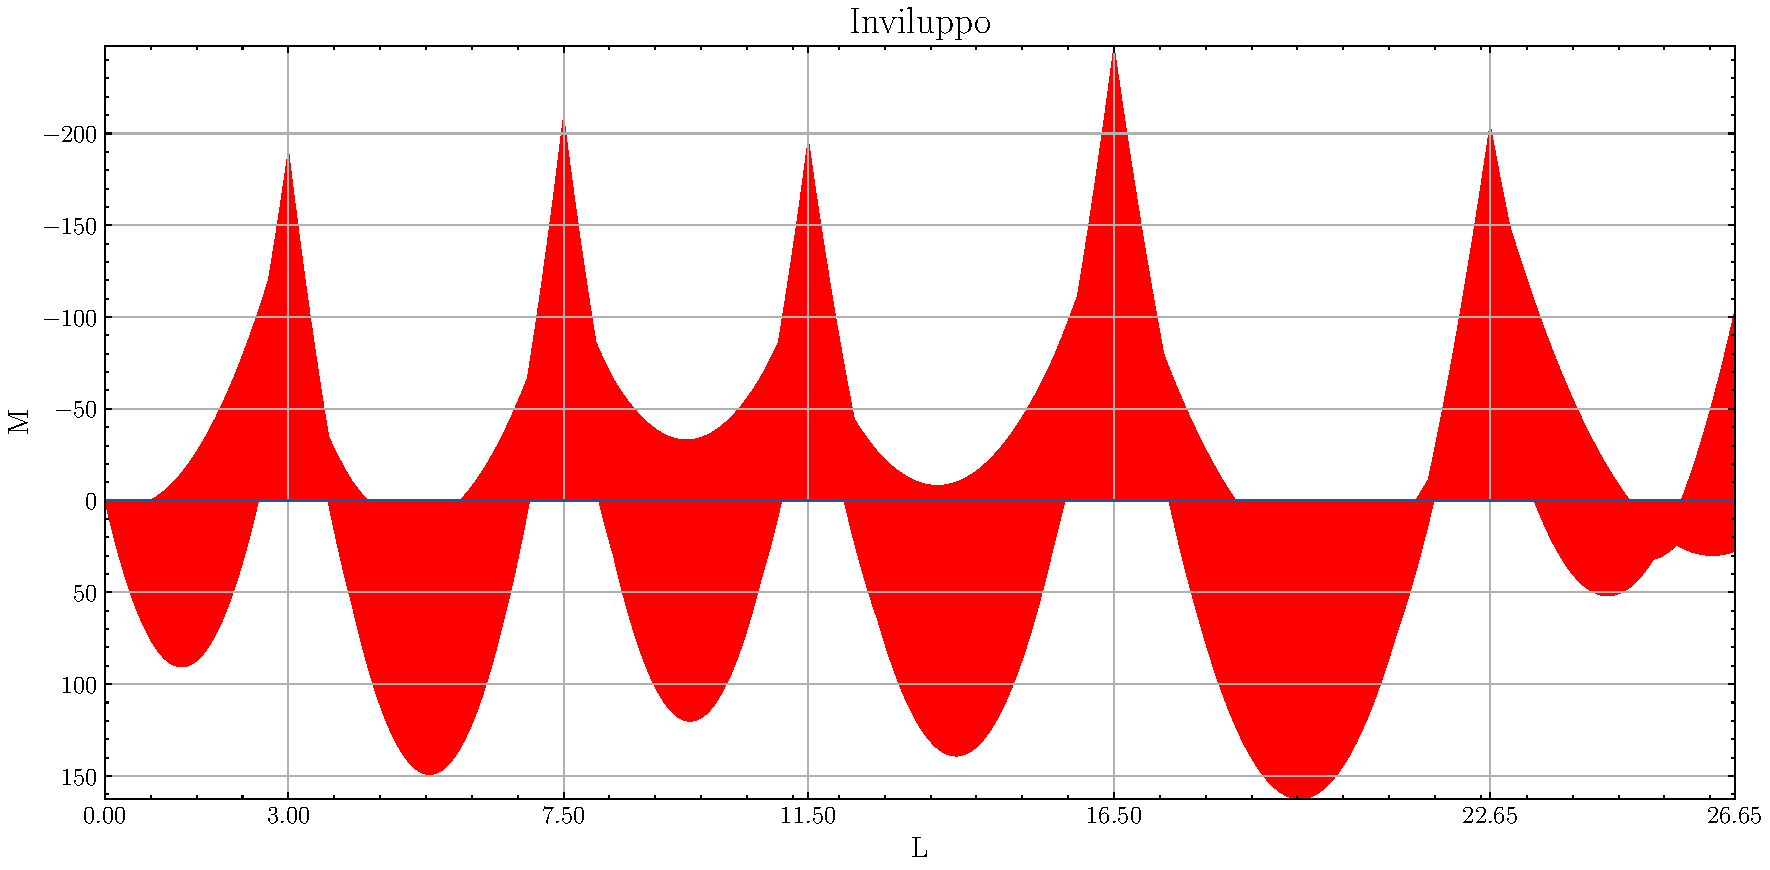
\includegraphics[height=0.6\textwidth]{IMG/diagrammi_trave/m.pdf}
\caption{Diagrammi del momento generati con combinazione di carico SLU}
\label{fig:trave_ULS_momento}
\end{figure}
\begin{table}[H]
\footnotesize
\centering
\caption{Valori del momento con combinazione di carico SLU nei punti più significativi della struttura}
\label{tab:trave_ULS_momento}
	\begin{tabular}{lS[table-format=-3.2]S[table-format=-3.2]S[table-format=-3.2]S[table-format=-3.2]S[table-format=-3.2]S[table-format=-3.2]S[table-format=-3.2]S[table-format=-3.2]S[table-format=-3.2]S[table-format=-3.2]S[table-format=-3.2]S[table-format=-3.2]S[table-format=-3.2]}
		\toprule
		{} & {A1} & {C1} & {A2} & {C2} & {A3} & {C3} & {A4} & {C4} & {A5} & {C5} & {A6} & {C6} & {A7} \\
		\midrule
		$s\,\si{[\metre]}$ & 0.00 & 1.26 & 3.00 & 5.31 & 7.50 & 9.57 & 11.50 & 13.92 & 16.50 & 19.54 & 22.65 & 24.57 & 26.65 \\
        $M^{-}\,\si{[\kilo\newton\metre]}$ & 0.00 & -15.14 & -190.97 & 0.00 & -209.46 & -33.15 & -196.60 & -10.06 & -247.45 & 0.00 & -204.82 & -18.04 & -103.04 \\
        $M^{+}\,\si{[\kilo\newton\metre]}$ & 0.00 & 90.60 & 0.00 & 149.18 & 0.00 & 120.20 & 0.00 & 139.16 & 0.00 & 162.53 & 0.00 & 51.88 & 27.68 \\
		\bottomrule
	\end{tabular}
\end{table}
\end{landscape}

%{} & {A1} & {C1} & {A2} & {C2} & {A3} & {C3} & {A4} & {C4} & {A5} & {C5} & {A6} & {C6} & {A7} \\
%&\multicolumn{1}{c}{Nodo 1}&\multicolumn{1}{c}{Camp. 1}&\multicolumn{1}{c}{Nodo 2}&\multicolumn{1}{c}{Camp. 2}&\multicolumn{1}{c}{Nodo 3}&\multicolumn{1}{c}{Camp. 3}&\multicolumn{1}{c}{Nodo 4}&\multicolumn{1}{c}{Camp. 4}&\multicolumn{1}{c}{Nodo 5}&\multicolumn{1}{c}{Camp. 5}&\multicolumn{1}{c}{Nodo 6}&\multicolumn{1}{c}{Camp. 6}&\multicolumn{1}{c}{Nodo 7}\\
		

\chapter{Materiali}
\chapter{Trave: momento flettente SLU}
\section{Progetto della sezione maggiormente sollecitata}
In riferimento ai valori mostrati in precedenza nella tabella \ref{tab:trave_ULS_momento} a pagina \pageref{tab:trave_ULS_momento}, si progetta ora la sezione in calcestruzzo armato considerando quella maggiormente sollecitata.
Nel caso in esame è quella in appoggio 5 avente un momento pari a $\SI{-247.45}{\kilo\newton\metre}$.
Essendo soggetta a momento flettente negativo, sarà considerata invertita rispetto la dispozione reale e considerata quindi a momento flettente positivo, con le amrature invertite. 
A tale scopo verrà utilizzata la nomenclatura \emph{inv.} nelle tabelle a seguire per indicare tutte quelle sezioni che sono state inveritite.

\begin{figure}[ht]
  \centering
  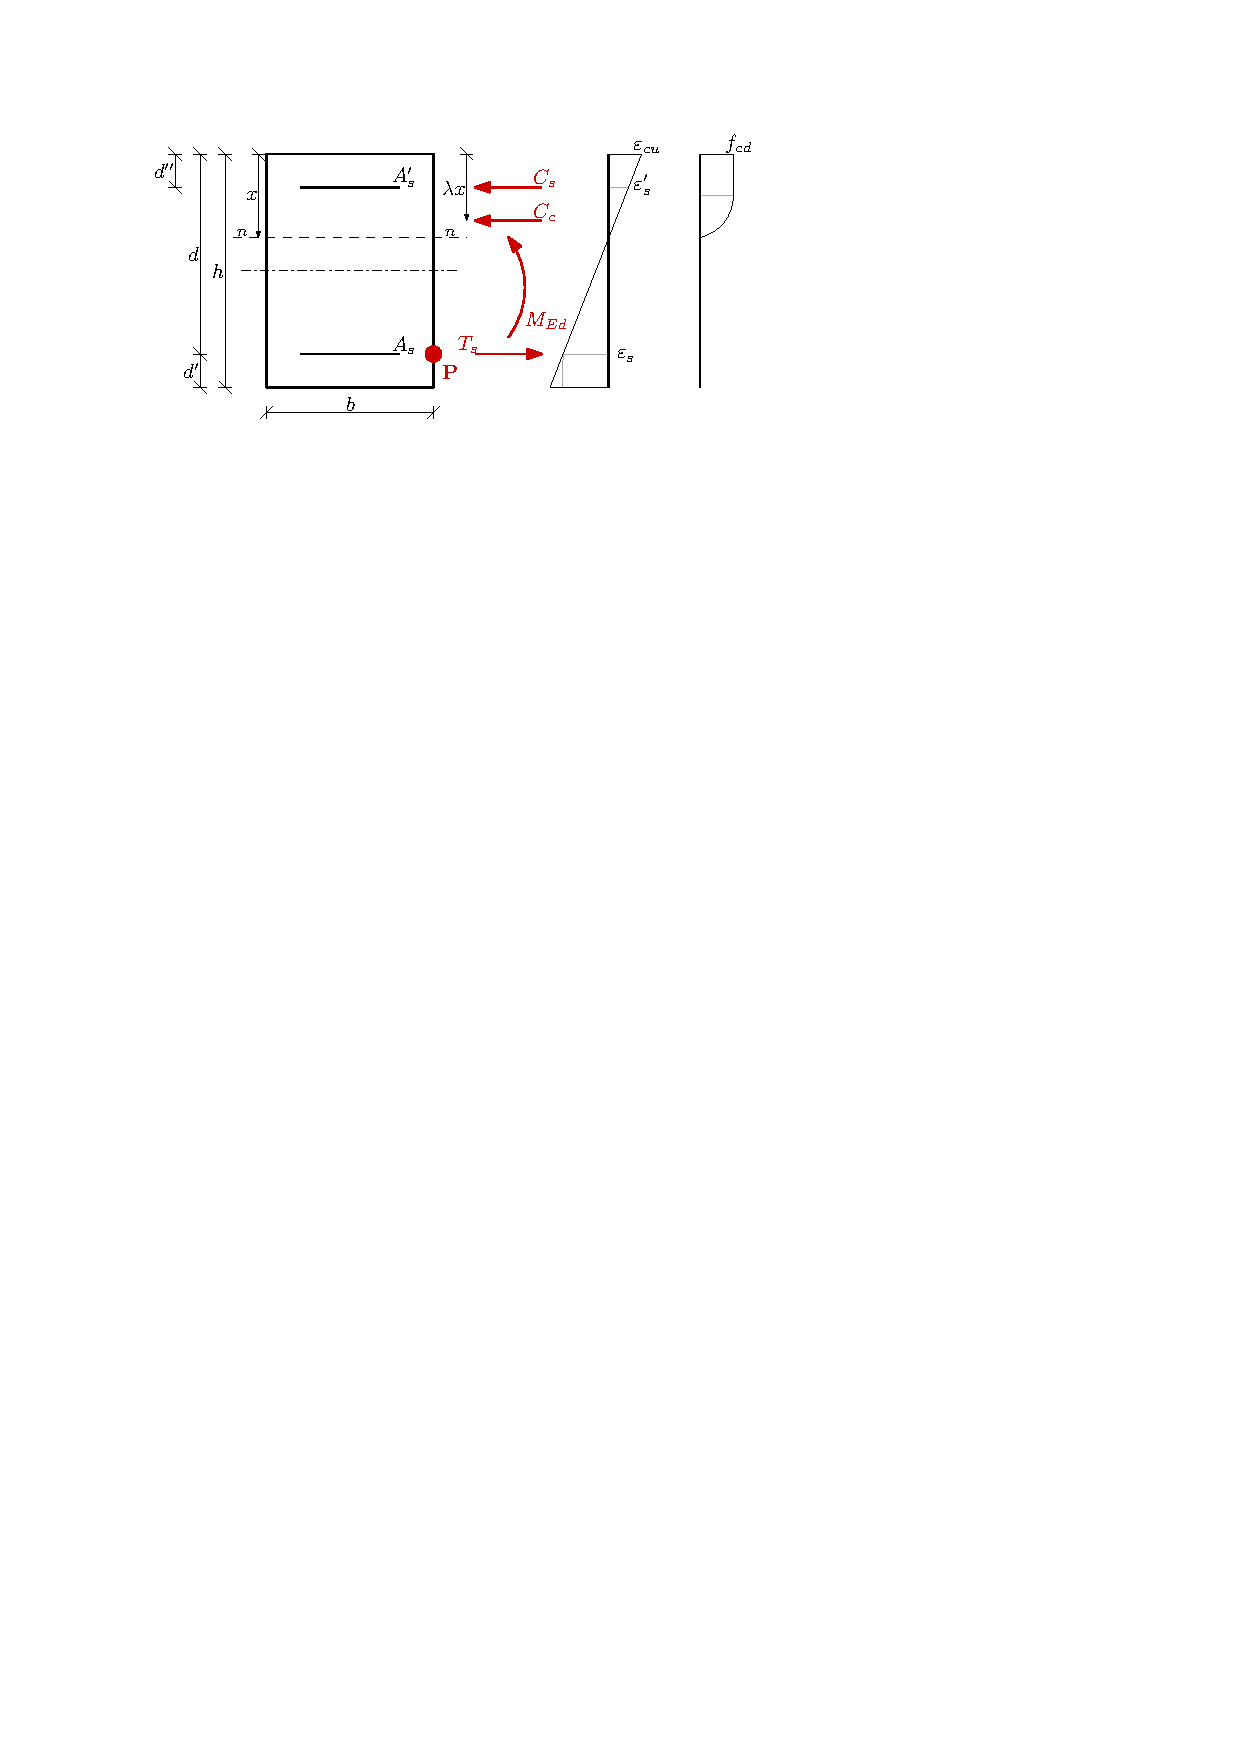
\includegraphics[height=0.25\textheight]{IMG/IPE_slu_progetto.pdf}
  \caption{Convenzione e nomenclatura utilizzata per il progetto agli SLU}
  \label{fig:slu_progetto}
\end{figure}

Utilizzando la convenzione di segni riportata in figura \ref{fig:slu_progetto} e il polo $\mathbf{P}$ riportato, è possibile scrivere il sistema per determinare i valori dell'altezza utile $d$ e della quantita di armature inferiori $A_s$ che soddisfano il momento flettente applicato. 
\begin{equation}
  \begin{cases}
    C_c + C_s - T_s = 0 \\
    C_c \left(d - \lambda\,x\right) + C_s \left(d - d^{\prime\prime}\right) = M_{Ed}
  \end{cases}
\end{equation}
Sistema che è possibile risolvere esplicitando i valori delle risultanti e facendo delle ipotesi per ridurrre il numero di variabili. 
Si fissa il rapporto di armatura $\beta = 0.2$, ovvero pari al minimo possibile, in quanto il momente flettente a segno opposto nella sezione in esame è nullo.
Inoltre il progetto è vincolato, pertanto la base è imposta a \SI{300}{\milli\metre}.
Come copriferri $d^\prime,d^{\prime\prime}$ si scelgono entrambi uguali e pari a \SI{40}{\milli\metre}.
Infine si fissa il pieno utilizzo delle capacità meccaniche dei materiali: per cui l'acciaio superiore risulta snervato, e di conseguenza $\sigma_s^\prime = f_{yd}$, e il calcestruzzo a collasso, e di conseguenza $\sigma_c = f_{cd}$.
I coefficienti $\lambda$ e $\psi$ sono quelli del campo 3 e quindi pari a $\frac{17}{21}$ e $\frac{99}{238}$.

Il sistema espanso risulta:
\begin{equation}
  \begin{cases}
    b \, \psi \, \xi \, d \, f_{cd} + \beta \, A_s \, f_{yd} - A_s \, f_{yd} = 0 \\
    b \, \psi \, \xi \, d \, f_{cd} \left(d - \lambda\,x\right) + \beta \, A_s \, f_{yd} \left(d - d^{\prime\prime}\right) = M_{Ed}
  \end{cases}
\end{equation}
e risolvendolo si ottengono i seguenti valori:
\begin{equation}
  \hookrightarrow \quad
  \begin{cases}
    A_s &= \SI{1416.82}{\milli\metre\squared} \\
    A_s^\prime &= \SI{283.36}{\milli\metre\squared} \\
    d &= \SI{497.23}{\milli\metre}
  \end{cases}
\end{equation}

Si vuole cercare di avere un'altezza totale $h = \SI{500}{\milli\metre}$, per cui si sceglie un'altezza utile $d = \SI{460}{\milli\metre}$ inferiore a quella ottenuta dal sistema. 
I valori di armature $A_s$ sono soddisfatti con ad esempio 8Ø16, 6Ø18 o 5Ø20, aventi rispettivamente \SI{1608}, \SI{1527}, \SI{1570}{\milli\metre\squared} di area.
Avendo problemi riguardo la base minima su cui si dispongono le barre, il diametro da 16 non può essere utilizzato. 
Vengono perciò adottati i 6Ø18 che rispettano i requisiti, come di seguito dimostrato:
\begin{equation}  
  \begin{split}
    b_{min} &= 2 \cdot \text{copriferro} + 2 \cdot \varnothing_\textup{staffe} + n_\textup{barre} \cdot \varnothing_\textup{barre} + \left( n_\textup{barre} - 1 \right) \cdot \text{dist}_\textup{barre}  \\
    &= 2 \cdot 20 + 2 \cdot 10 + 6 \cdot 18 + \left( 6 - 1 \right) \cdot 25 \quad \si{\milli\metre}\\
    &= \SI{293}{\milli\metre} < b = \SI{300}{\milli\metre} \quad \checkmark ,
  \end{split}
\end{equation}
mentre per le armature superiori si scelgono 2Ø18 con unica funzione di reggistaffa.

\subsection{Verifica della sezione maggiormente sollecitata}
%--- LOG --- 
%Ipotesi di campo 3B, calcolo della retta limite 2-3
%xi_23 = 0.25926
%Esiste campo 2a, 2b, 3b perchè d2 = 40.00 < d2_xi23 = 55.77 mm
%xi_3 = 0.25166
%Ipotesi di campo 3 errata! xi_3 = 0.25166 < xi_23 = 0.25926 ma devo comunque verificare tramite es1 perché ho usato hp di es plasticizzato del 3B
%Essendo d2 = 40.00000 < d2_xi23 = 55.76720, non può esserci il campo 3A
%Calcolo xi con ipotesi di campo 2B: armature superiori snervate
%xi_2b = 0.25349
%!!!!!!!!!!!!!!verifica del ec da fare
%Ipotesi armature superiori snervate ok! es1 = 0.22308% > di ese1 = 0.18634%

%campo': '2B',
% 'ec': 0.0033956711163810735,
% 'es': 0.01,
% 'es1': 0.002230830149739241,
% 'xi': 0.2534901825283417,
% 'psi': 0.8036716031035525,
% 'lamb': 0.4138260346516767,
% 'Nrd': 0.0,
% 'Mrd': 247633547.16419485

  \begin{table}[htb]
    \centering
    \scriptsize
    \caption{ULS}
    \begin{tabular}{
        l
        c
        c
        S[table-format=3.3]
        l
        S[table-format=2.2]
        S[table-format=2.2]
        S[table-format=2.2]
        S[table-format=1.4]
        S[table-format=1.4]
        S[table-format=1.4]
        S[table-format=3.3]
        r
        S[table-format=2.1]}
    \toprule
    \multirow{2}{*}{Sez.}   & \multirow{2}{*}{$A_s$}    & \multirow{2}{*}{$A_s^\prime$} & {$M_{Ed}$}                    & \multirow{2}{*}{Campo}    & {$\varepsilon_c$}         & {$\varepsilon_s$}         & {$\varepsilon_s^\prime$}  & \multicolumn{1}{c}{\multirow{2}{*}{$\xi$}}    & \multicolumn{1}{c}{\multirow{2}{*}{$\psi$}}   & \multicolumn{1}{c}{\multirow{2}{*}{$\lambda$}}    & {$M_{Rd}$}                    & \multicolumn{2}{l}{$M_{Ed}<M_{Rd}$} \\
                            &                           &                               & {\si{[\kilo\newton\metre]}}   &                           &{\si{[\textperthousand]}}  &{\si{[\textperthousand]}}  &  {\si{[\textperthousand]}} &                        &                           &                               & {\si{[\kilo\newton\metre]}}   & & {\si{[\percent]}}\\
    \midrule
    A1 inv & 2Ø18 & 2Ø18 & 0.000   & 2A-1 & 1.51 & 10.00 & 0.51 & 0.1311 & 0.5648 & 0.3613 & 86.276  & \checkmark & 0.0 \\
    C1     & 3Ø18 & 2Ø18 & 90.595  & 2A-1 & 1.91 & 10.00 & 0.88 & 0.1607 & 0.6519 & 0.3724 & 128.015 & \checkmark & 70.8 \\
    A2 inv & 6Ø18 & 2Ø18 & 190.969 & 2B   & 3.40 & 10.00 & 2.23 & 0.2535 & 0.8037 & 0.4138 & 247.634 & \checkmark & 77.1 \\
    C2     & 4Ø18 & 2Ø18 & 149.180 & 2A-2 & 2.33 & 10.00 & 1.26 & 0.1890 & 0.7139 & 0.3856 & 168.988 & \checkmark & 88.3 \\
    A3 inv & 6Ø18 & 2Ø18 & 209.462 & 2B   & 3.40 & 10.00 & 2.23 & 0.2535 & 0.8037 & 0.4138 & 247.634 & \checkmark & 84.6 \\
    C3     & 3Ø18 & 2Ø18 & 120.204 & 2A-1 & 1.91 & 10.00 & 0.88 & 0.1607 & 0.6519 & 0.3724 & 128.015 & \checkmark & 93.9 \\
    A4 inv & 6Ø18 & 2Ø18 & 196.601 & 2B   & 3.40 & 10.00 & 2.23 & 0.2535 & 0.8037 & 0.4138 & 247.634 & \checkmark & 79.4 \\
    C4     & 4Ø18 & 2Ø18 & 139.165 & 2A-2 & 2.33 & 10.00 & 1.26 & 0.1890 & 0.7139 & 0.3856 & 168.988 & \checkmark & 82.4 \\
    A5 inv & 6Ø18 & 2Ø18 & 247.450 & 2B   & 3.40 & 10.00 & 2.23 & 0.2535 & 0.8037 & 0.4138 & 247.634 & \checkmark & 99.9 \\
    C5     & 4Ø18 & 2Ø18 & 162.530 & 2A-2 & 2.33 & 10.00 & 1.26 & 0.1890 & 0.7139 & 0.3856 & 168.988 & \checkmark & 96.2 \\
    A6 inv & 6Ø18 & 2Ø18 & 204.824 & 2B   & 3.40 & 10.00 & 2.23 & 0.2535 & 0.8037 & 0.4138 & 247.634 & \checkmark & 82.7 \\
    C6     & 2Ø18 & 2Ø18 & 51.884  & 2A-1 & 1.51 & 10.00 & 0.51 & 0.1311 & 0.5648 & 0.3613 & 86.276  & \checkmark & 60.1 \\
    A7 inv & 3Ø18 & 2Ø18 & 103.039 & 2A-1 & 1.91 & 10.00 & 0.88 & 0.1607 & 0.6519 & 0.3724 & 128.015 & \checkmark & 80.5 \\
    \midrule
    A1     & 2Ø18 & 2Ø18 & 0.000   & 2A-1 & 1.51 & 10.00 & 0.51 & 0.1311 & 0.5648 & 0.3613 & 86.276  & \checkmark & 0.0 \\
    C1 inv & 2Ø18 & 3Ø18 & 15.137  & 2A-1 & 1.42 & 10.00 & 0.42 & 0.1241 & 0.5410 & 0.3591 & 86.200  & \checkmark & 17.6 \\
    A2     & 2Ø18 & 6Ø18 & 0.000   & 2A-1 & 1.26 & 10.00 & 0.28 & 0.1119 & 0.4978 & 0.3555 & 86.004  & \checkmark & 0.0 \\
    C2 inv & 2Ø18 & 4Ø18 & 0.000   & 2A-1 & 1.35 & 10.00 & 0.36 & 0.1189 & 0.5230 & 0.3575 & 86.126  & \checkmark & 0.0 \\
    A3     & 2Ø18 & 6Ø18 & 0.000   & 2A-1 & 1.26 & 10.00 & 0.28 & 0.1119 & 0.4978 & 0.3555 & 86.004  & \checkmark & 0.0 \\
    C3 inv & 2Ø18 & 3Ø18 & 33.154  & 2A-1 & 1.42 & 10.00 & 0.42 & 0.1241 & 0.5410 & 0.3591 & 86.200  & \checkmark & 38.5 \\
    A4     & 2Ø18 & 6Ø18 & 0.000   & 2A-1 & 1.26 & 10.00 & 0.28 & 0.1119 & 0.4978 & 0.3555 & 86.004  & \checkmark & 0.0 \\
    C4 inv & 2Ø18 & 4Ø18 & 10.062  & 2A-1 & 1.35 & 10.00 & 0.36 & 0.1189 & 0.5230 & 0.3575 & 86.126  & \checkmark & 11.7 \\
    A5     & 2Ø18 & 6Ø18 & 0.000   & 2A-1 & 1.26 & 10.00 & 0.28 & 0.1119 & 0.4978 & 0.3555 & 86.004  & \checkmark & 0.0 \\
    C5 inv & 2Ø18 & 4Ø18 & 0.000   & 2A-1 & 1.35 & 10.00 & 0.36 & 0.1189 & 0.5230 & 0.3575 & 86.126  & \checkmark & 0.0 \\
    A6     & 2Ø18 & 6Ø18 & 0.000   & 2A-1 & 1.26 & 10.00 & 0.28 & 0.1119 & 0.4978 & 0.3555 & 86.004  & \checkmark & 0.0 \\
    C6 inv & 2Ø18 & 2Ø18 & 18.039  & 2A-1 & 1.51 & 10.00 & 0.51 & 0.1311 & 0.5648 & 0.3613 & 86.276  & \checkmark & 20.9 \\
    A7     & 2Ø18 & 3Ø18 & 27.682  & 2A-1 & 1.42 & 10.00 & 0.42 & 0.1241 & 0.5410 & 0.3591 & 86.200  & \checkmark & 32.1 \\
    \bottomrule
    \end{tabular}
    \end{table}

\end{document} 